\documentclass{standalone}
\usepackage{tikz}
\usetikzlibrary{patterns, positioning}
\usepackage[sfdefault]{ClearSans} %% option 'sfdefault' activates Clear Sans as the default text font
\usepackage[T1]{fontenc}

\begin{document}
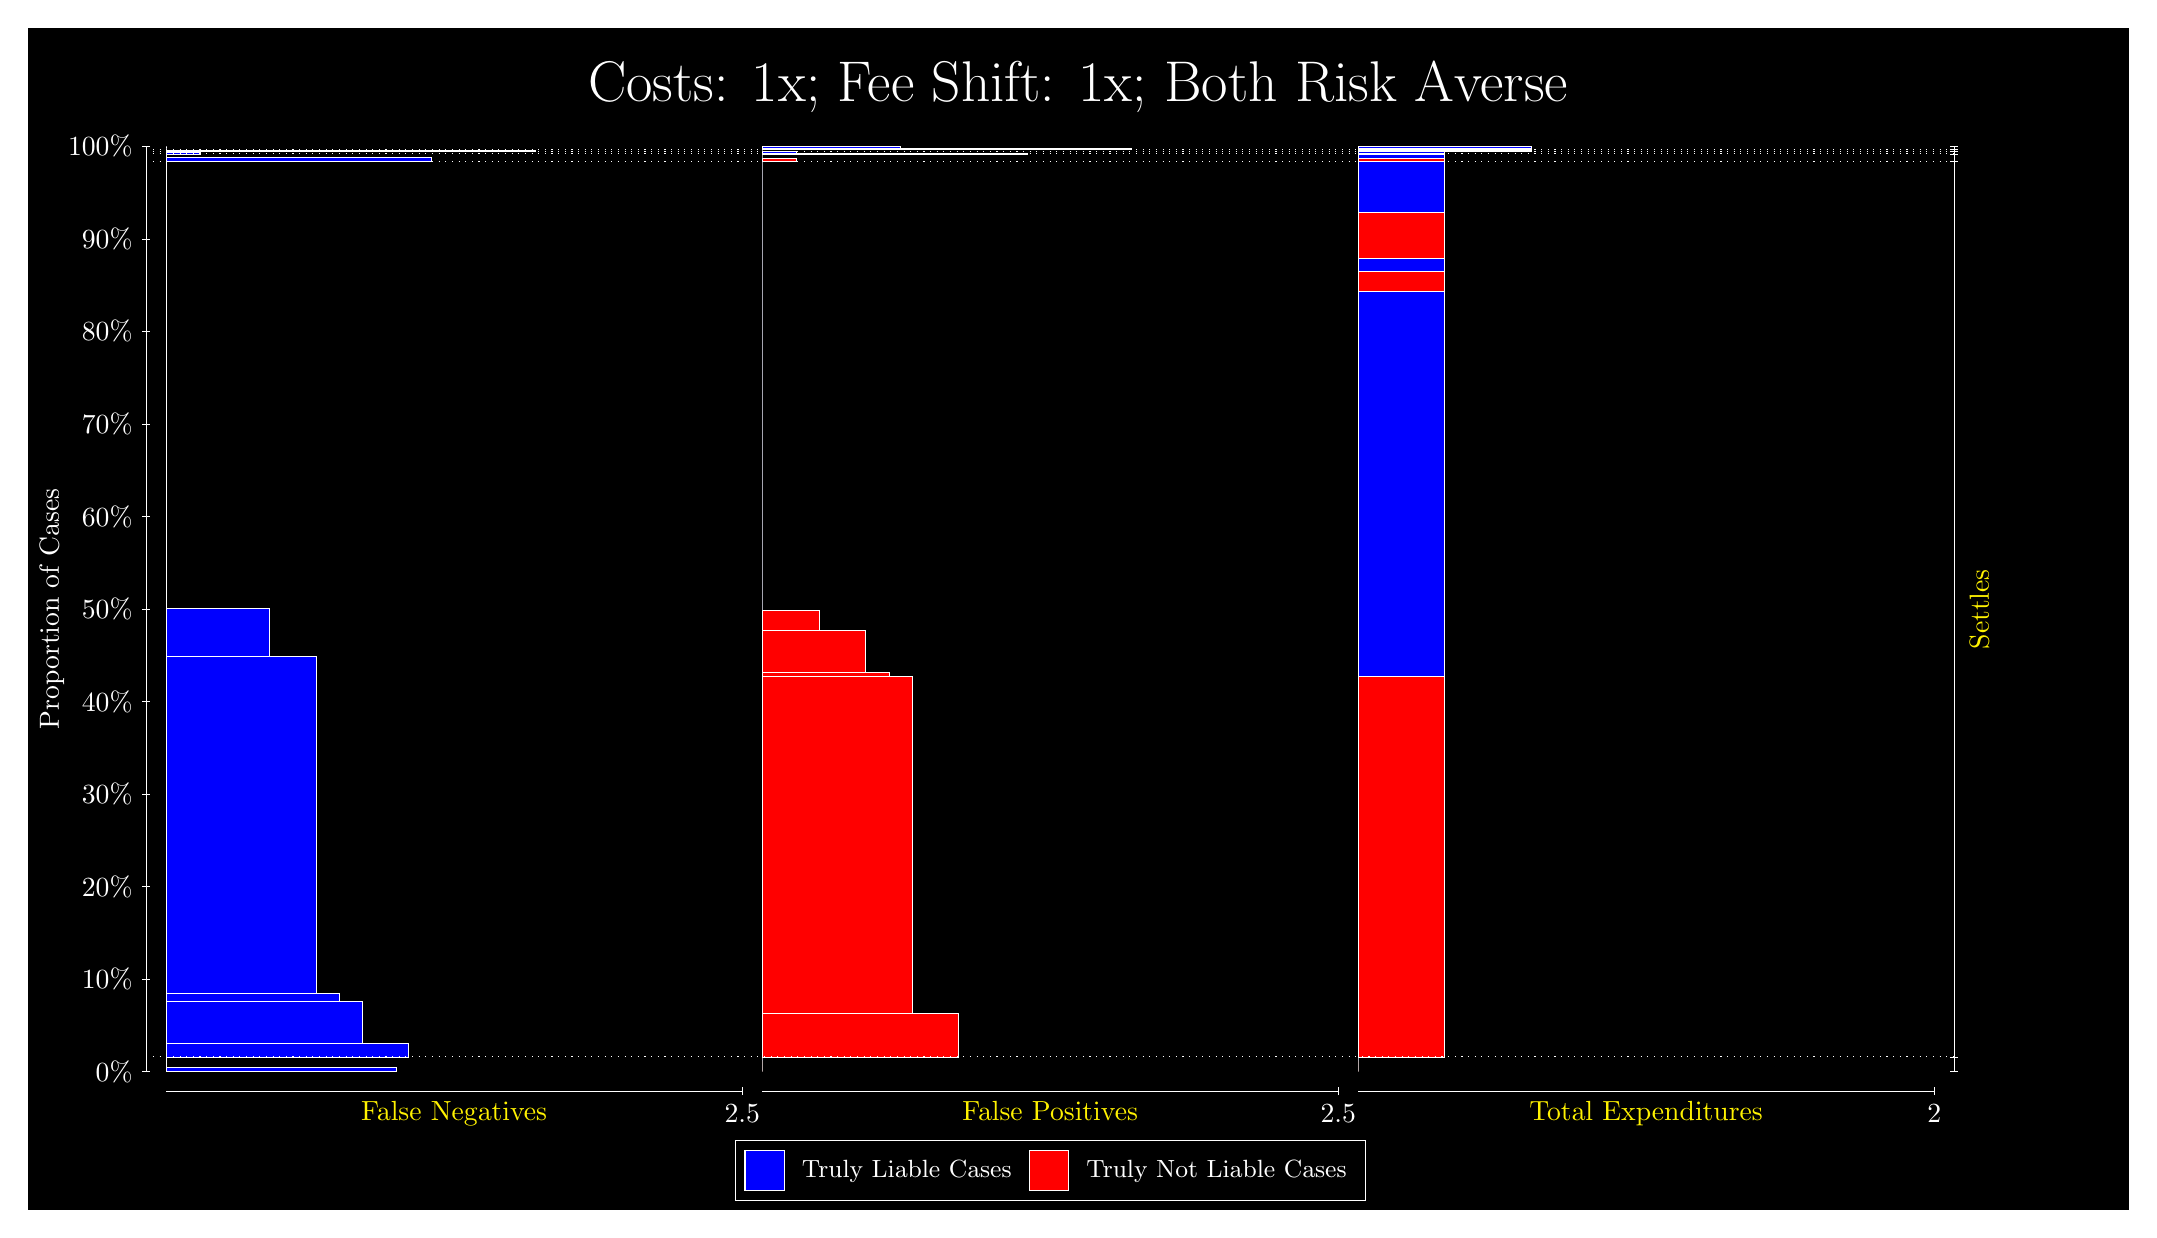
\begin{tikzpicture}
\draw[fill=black] (0,0) rectangle (26.667,15);
\draw[text=white] (0,13.5) rectangle (26.667,15) node[midway] {\huge Costs: 1x; Fee Shift: 1x; Both Risk Averse};
\draw[white, very thin] (1.5,1.75) -- (1.5,13.5);
\node[rotate=90, text=white, anchor=center] at (0.3, 7.625) {Proportion of Cases};
\draw[white, very thin] (1.45,1.75) -- (1.55,1.75);
\node[text=white, anchor=east] at (1.45, 1.75) {0\%};
\draw[white, very thin] (1.45,2.925) -- (1.55,2.925);
\node[text=white, anchor=east] at (1.45, 2.925) {10\%};
\draw[white, very thin] (1.45,4.1) -- (1.55,4.1);
\node[text=white, anchor=east] at (1.45, 4.1) {20\%};
\draw[white, very thin] (1.45,5.275) -- (1.55,5.275);
\node[text=white, anchor=east] at (1.45, 5.275) {30\%};
\draw[white, very thin] (1.45,6.45) -- (1.55,6.45);
\node[text=white, anchor=east] at (1.45, 6.45) {40\%};
\draw[white, very thin] (1.45,7.625) -- (1.55,7.625);
\node[text=white, anchor=east] at (1.45, 7.625) {50\%};
\draw[white, very thin] (1.45,8.8) -- (1.55,8.8);
\node[text=white, anchor=east] at (1.45, 8.8) {60\%};
\draw[white, very thin] (1.45,9.975) -- (1.55,9.975);
\node[text=white, anchor=east] at (1.45, 9.975) {70\%};
\draw[white, very thin] (1.45,11.15) -- (1.55,11.15);
\node[text=white, anchor=east] at (1.45, 11.15) {80\%};
\draw[white, very thin] (1.45,12.325) -- (1.55,12.325);
\node[text=white, anchor=east] at (1.45, 12.325) {90\%};
\draw[white, very thin] (1.45,13.5) -- (1.55,13.5);
\node[text=white, anchor=east] at (1.45, 13.5) {100\%};

\draw[white, very thin] (24.457,1.75) -- (24.457,13.5);
\draw[white, very thin] (24.407,1.75) -- (24.507,1.75);
\node[anchor=west] at (24.407, 1.75) {};
\draw[white, very thin] (24.407,1.9368) -- (24.507,1.9368);
\node[anchor=west] at (24.407, 1.9368) {};
\draw[white, very thin] (24.407,13.304) -- (24.507,13.304);
\node[anchor=west] at (24.407, 13.304) {};
\draw[white, very thin] (24.407,13.404) -- (24.507,13.404);
\node[anchor=west] at (24.407, 13.404) {};
\draw[white, very thin] (24.407,13.433) -- (24.507,13.433);
\node[anchor=west] at (24.407, 13.433) {};
\draw[white, very thin] (24.407,13.462) -- (24.507,13.462);
\node[anchor=west] at (24.407, 13.462) {};
\draw[white, very thin] (24.407,13.5) -- (24.507,13.5);
\node[anchor=west] at (24.407, 13.5) {};

\draw[white, very thin, fill=blue] (1.75,1.75) rectangle (4.6775,1.8013);
\draw[white, very thin, fill=red] (1.75,1.8013) rectangle (1.75,1.9368);
\draw[white, very thin, fill=blue] (1.75,1.9368) rectangle (4.8239,2.1084);
\draw[white, very thin, fill=blue] (1.75,2.1084) rectangle (4.2384,2.6425);
\draw[white, very thin, fill=blue] (1.75,2.6425) rectangle (3.9457,2.7459);
\draw[white, very thin, fill=blue] (1.75,2.7459) rectangle (3.6529,7.0186);
\draw[white, very thin, fill=blue] (1.75,7.0186) rectangle (3.0674,7.6388);
\draw[white, very thin, fill=red] (1.75,7.6388) rectangle (1.75,13.304);
\draw[white, very thin, fill=blue] (1.75,13.304) rectangle (5.1167,13.361);
\draw[white, very thin, fill=red] (1.75,13.361) rectangle (1.75,13.404);
\draw[white, very thin, fill=blue] (1.75,13.404) rectangle (2.1891,13.426);
\draw[white, very thin, fill=red] (1.75,13.426) rectangle (1.75,13.433);
\draw[white, very thin, fill=blue] (1.75,13.433) rectangle (6.4341,13.448);
\draw[white, very thin, fill=red] (1.75,13.448) rectangle (1.75,13.462);
\draw[white, very thin, fill=red] (1.75,13.462) rectangle (1.75,13.472);
\draw[white, very thin, fill=blue] (1.75,13.472) rectangle (1.75,13.5);
\draw[white, very thin, fill=red] (9.3189,1.75) rectangle (9.3189,1.8855);
\draw[white, very thin, fill=blue] (9.3189,1.8855) rectangle (9.3189,1.9368);
\draw[white, very thin, fill=red] (9.3189,1.9368) rectangle (11.807,2.4918);
\draw[white, very thin, fill=red] (9.3189,2.4918) rectangle (11.222,6.7645);
\draw[white, very thin, fill=red] (9.3189,6.7645) rectangle (10.929,6.8176);
\draw[white, very thin, fill=red] (9.3189,6.8176) rectangle (10.636,7.3517);
\draw[white, very thin, fill=red] (9.3189,7.3517) rectangle (10.051,7.602);
\draw[white, very thin, fill=blue] (9.3189,7.602) rectangle (9.3189,13.304);
\draw[white, very thin, fill=red] (9.3189,13.304) rectangle (9.758,13.347);
\draw[white, very thin, fill=blue] (9.3189,13.347) rectangle (9.3189,13.404);
\draw[white, very thin, fill=red] (9.3189,13.404) rectangle (12.686,13.41);
\draw[white, very thin, fill=blue] (9.3189,13.41) rectangle (9.758,13.433);
\draw[white, very thin, fill=red] (9.3189,13.433) rectangle (9.3189,13.448);
\draw[white, very thin, fill=blue] (9.3189,13.448) rectangle (9.3189,13.462);
\draw[white, very thin, fill=red] (9.3189,13.462) rectangle (14.003,13.472);
\draw[white, very thin, fill=blue] (9.3189,13.472) rectangle (11.075,13.5);
\draw[white, very thin, fill=red] (16.888,1.75) rectangle (16.888,1.8855);
\draw[white, very thin, fill=blue] (16.888,1.8855) rectangle (16.888,1.9368);
\draw[white, very thin, fill=red] (16.888,1.9368) rectangle (17.986,6.7645);
\draw[white, very thin, fill=blue] (16.888,6.7645) rectangle (17.986,11.657);
\draw[white, very thin, fill=red] (16.888,11.657) rectangle (17.986,11.908);
\draw[white, very thin, fill=blue] (16.888,11.908) rectangle (17.986,12.079);
\draw[white, very thin, fill=red] (16.888,12.079) rectangle (17.986,12.667);
\draw[white, very thin, fill=blue] (16.888,12.667) rectangle (17.986,13.304);
\draw[white, very thin, fill=red] (16.888,13.304) rectangle (17.986,13.347);
\draw[white, very thin, fill=blue] (16.888,13.347) rectangle (17.986,13.404);
\draw[white, very thin, fill=red] (16.888,13.404) rectangle (17.986,13.41);
\draw[white, very thin, fill=blue] (16.888,13.41) rectangle (17.986,13.433);
\draw[white, very thin, fill=red] (16.888,13.433) rectangle (19.083,13.448);
\draw[white, very thin, fill=blue] (16.888,13.448) rectangle (19.083,13.462);
\draw[white, very thin, fill=red] (16.888,13.462) rectangle (19.083,13.472);
\draw[white, very thin, fill=blue] (16.888,13.472) rectangle (19.083,13.5);
\draw[white, dotted] (1.5,1.9368) -- (24.457,1.9368);
\draw[white, dotted] (1.5,13.304) -- (24.457,13.304);
\draw[white, dotted] (1.5,13.404) -- (24.457,13.404);
\draw[white, dotted] (1.5,13.433) -- (24.457,13.433);
\draw[white, dotted] (1.5,13.462) -- (24.457,13.462);
\draw[white, very thin] (1.75,1.5) -- (9.0689,1.5);
\node[text=yellow, anchor=north] at (5.4094, 1.5) {False Negatives};
\draw[white, very thin] (9.0689,1.45) -- (9.0689,1.55);
\node[text=white, anchor=north] at (9.0689, 1.45) {2.5};

\draw[white, very thin] (9.3189,1.5) -- (16.638,1.5);
\node[text=yellow, anchor=north] at (12.978, 1.5) {False Positives};
\draw[white, very thin] (16.638,1.45) -- (16.638,1.55);
\node[text=white, anchor=north] at (16.638, 1.45) {2.5};

\draw[white, very thin] (16.888,1.5) -- (24.207,1.5);
\node[text=yellow, anchor=north] at (20.547, 1.5) {Total Expenditures};
\draw[white, very thin] (24.207,1.45) -- (24.207,1.55);
\node[text=white, anchor=north] at (24.207, 1.45) {2};


\node[text=yellow, centered, rotate=90] at (24.777, 7.6204) {Settles};





\draw (12.978300999999998,1.5) node[draw=none] (baseCoordinate) {};
\begin{scope}[align=center]
        \matrix[scale=0.5, draw=white, below=0.5cm of baseCoordinate, nodes={draw}, column sep=0.1cm]{
            \node[rectangle, draw, minimum width=0.5cm, minimum height=0.5cm, fill=blue] {}; &
            \node[draw=none, font=\small, text=white] (B) {Truly Liable Cases}; &
            \node[rectangle, draw, minimum width=0.5cm, minimum height=0.5cm, fill=red] {}; &
            \node[draw=none, font=\small, text=white] (B) {Truly Not Liable Cases}; \\
            };
\end{scope}

\end{tikzpicture}
\end{document}